% !TEX program = xelatex
\documentclass[11pt,a4paper]{ctexart}

% --- 页面与排版宏包 ---
\usepackage[a4paper,top=2.2cm,bottom=2.2cm,left=2.2cm,right=2.2cm]{geometry}
\usepackage{amsmath,amssymb,amsthm}
\usepackage{booktabs,array,tabularx,multirow}
\usepackage{graphicx}
\usepackage{xcolor}
\usepackage{tikz}
\usetikzlibrary{arrows.meta,positioning,shapes.geometric,fit}
\usepackage{enumitem}
\usepackage{float}
\usepackage[most]{tcolorbox}
\usepackage[hidelinks,colorlinks=true,linkcolor=blue!55!black,citecolor=teal!60!black,urlcolor=blue!65!black]{hyperref}
\usepackage{xurl}
\usepackage{fancyhdr}

% --- 页眉页脚设置 ---
\pagestyle{fancy}
\fancyhf{}
\fancyhead[L]{\small\color{gray!70!black} 长城科研共同体 V6-Up (v3.0.0) · 第 7 轮实机测试科研实验报告}
\fancyhead[R]{\small\color{gray!70!black} 2026 年 11 月}
\fancyfoot[C]{\small\thepage}
\renewcommand{\headrulewidth}{0.4pt}

% --- 定理与环境定义 ---
\newtheorem{theorem}{定理}[section]
\newtheorem{proposition}[theorem]{命题}
\theoremstyle{remark}
\newtheorem{remark}[theorem]{注记}

% --- 实录展示框样式 ---
\tcbset{
    dialoguebox/.style={
        enhanced,
        colback=blue!2!white,
        colframe=blue!45!black,
        boxrule=0.6pt,
        arc=2pt,
        left=6pt,right=6pt,top=5pt,bottom=5pt,
        fonttitle=\small\bfseries,
        coltitle=white,
        colbacktitle=blue!50!black,
        breakable
    }
}

% --- 列表间距微调 ---
\setlist[itemize]{itemsep=2pt,parsep=1pt,topsep=4pt}
\setlist[enumerate]{itemsep=2pt,parsep=1pt,topsep=4pt}

% --- 标题信息 ---
\title{\textbf{长城科研共同体 V6-Up (v3.0.0) 第 7 轮实机测试实验报告} \\[0.35em]
\large ——基于 v3.0 顶层架构白皮书的全流程实证复盘与收敛/算力重心分析}
\author{实验系统：DeepSeek Harness (0.2.2-rc.5) $\times$ Python Single-Writer 控制面 \\
实验数据根目录：\texttt{D:\textbackslash Documents\textbackslash deepseek\allowbreak\ harness\textbackslash\allowbreak v6第七轮测试}}
\date{2026 年 11 月 22 日}

\begin{document}

\maketitle

\begin{abstract}
严格依据《长城 Agent V6-Up 架构白皮书（v3.0）》 系统介绍本多智能体自主科研系统的第一性原理与制度设计，并全面汇报第 7 轮端到端实机测试的真实运行过程、有效科学产出、典型交互案例与核心问题诊断。本轮测试以 2026 年高教社杯全国大学生数学建模竞赛 B 题（无线电干扰源的快速自动定位与清除，Q1--Q4）为验证课题，于 2026 年 11 月 22 日 20:12（UTC+8，下同）启动；期间虽于 21:50--22:13 遭遇 Q2 采样脚本内存失控导致的宿主崩溃，但在主控签发 R1 护栏裁决与修复重启后系统恢复并行推进，直至 22:36:50--22:44:11 因\textbf{外部 API 账户额度耗尽（HTTP 402 \texttt{ACCOUNT\_QUOTA: Insufficient Balance}）}而被迫全面停机（后台治理唤醒延续至 23:07:29），最终停留在 \path{STAGE2_EVOLVE} 阶段。

尽管实验因额度耗尽而中途停止（若非余额耗尽，修复护栏后的系统本可继续长周期运行），本轮实测在系统工程与科学发现上均已取得扎实进展：(1) \textbf{v3.0 核心架构全面跑通}：极薄事件总线、一委三部扁平制衡、“3 真相 + 2 视图”控制面、双向沙箱平权与科研仪器科三档四态机制均在 100 个子会话并发中得到真实兑现，沉淀 2,019 条知识图谱边、14 份定额重压缩看板（1,144--1,887 字符，100\% 遵守 $\le 2200$ 字上限）、24 条独立死胡同记录与 13 次全通过审计；(2) \textbf{Q1 可用级别}：历经 3 次独立盲审（含 \texttt{rev\_001} 退回重修），入账 2 项 \path{FULL_GOAL} 级 \path{L3_VERIFIED} 定理（\path{L3-001}、\path{L3-002}），完整证伪直径圆覆盖猜想；(3) \textbf{找准问题重心（收敛与算力）}：系统已实际进入 Q2 并重起两条正交学派，但 Q1 在达成 \path{FULL_GOAL} 后仍保留 3 路冗余并行，与 Q2 共同撞上 5 并发 API 限流并加速耗尽账户余额。围绕“如何及时收敛止盈与管控算力配额”，报告提出了第 8 轮重启的明确改进路线。

\medskip
\noindent\textbf{关键词：} 长城 Agent V6-Up；一委三部；3 真相 2 视图；沙箱平权；问题收敛；算力控制
\end{abstract}

\tableofcontents
\newpage

% =====================================================================
\section{系统架构全景：基于 v3.0 顶层白皮书的组织机理}
% =====================================================================

针对大模型从“单轮代码生成”迈向“10--20 小时、高并发、无人值守自主科学发现”时必然爆发的四大结构性病灶——\textbf{① 长上下文注意力退化与“虚假繁荣”停滞、② 高并发下的群体思维坍塌（Diversity Collapse）、③ 非标量化科学问题的“梯度缺失”与路灯效应、④ 静态验证脚手架天花板与评测器自身缺陷}——长城 Agent V6-Up (v3.0) 确立了一套以\textbf{“极薄无偏见事件总线 $\times$ 一委三部扁平制衡 $\times$ 3 真相 + 2 视图 $\times$ 沙箱平权 $\times$ 科研仪器科”}为核心的制度化科研共同体架构（见图~\ref{fig:arch}）。



在会话拓扑上，系统摒弃“大总管长期常驻 + 父子派单树”，采用\textbf{极薄确定性事件总线（DSH Control Plane）+ 全员短生命周期会话}：5 个治理角色每次唤醒均为独立一次性无状态短会话（写库即销毁）；一线探索单元的 1 对 1 伴随助手仅在\textbf{单个探索节点内部}暂停续传（节点完结即随探索者一同销毁，绝不跨代常驻），且\textbf{严禁在工作区磁盘生成任何过程审批、汇报或审计类 \texttt{.md} 公文}。

\begin{figure}[htbp]
\centering
\begin{tikzpicture}[
    node distance=0.55cm and 0.45cm,
    box/.style={rectangle, draw=blue!55!black, fill=blue!4, rounded corners=3pt, text width=2.85cm, align=center, font=\scriptsize, minimum height=1.0cm},
    gov/.style={rectangle, draw=teal!60!black, fill=teal!5, rounded corners=3pt, text width=2.75cm, align=center, font=\scriptsize, minimum height=0.95cm},
    dbbox/.style={rectangle, draw=orange!65!black, fill=orange!6, rounded corners=3pt, text width=4.2cm, align=center, font=\scriptsize, minimum height=1.25cm},
    sbx/.style={rectangle, draw=purple!55!black, fill=purple!4, rounded corners=3pt, text width=4.0cm, align=center, font=\scriptsize, minimum height=1.25cm},
    arrow/.style={-{Stealth[length=2mm]}, semithick, color=gray!65!black}
]
% 顶层：人类与确定性总线
\node[gov, text width=3.3cm] (user) {\textbf{人类科研者 / 主控}\\签发 Parse 0 六项表单\\与补充裁决 (\texttt{rulings/})};
\node[box, right=0.9cm of user, text width=4.8cm] (bus) {\textbf{DSH 确定性极薄事件总线 (\texttt{0.2.2-rc.5})}\\零权力/零科学偏见 · 监听 37\%/70\% 水位、分诊、\\盲审、工单与 >50\% 聚拢 · 输出右侧栏遥测面板};

% 中层：一线探索单元 + 一委三部
\node[box, below=0.85cm of user, xshift=-0.6cm] (exp) {\textbf{前沿探索者}\\(\texttt{explorer})\\独立 Worktree · 37\%/70\% 时钟};
\node[box, right=0.35cm of exp] (comp) {\textbf{1 对 1 伴随助手}\\(\texttt{lineage\_companion})\\单节点续传 · 独占写 DAG};
\node[gov, right=0.35cm of comp] (ver) {\textbf{中央图书馆 · 盲审官}\\(\texttt{library\_verifier})\\空白沙箱两阶段实测裁决};
\node[gov, right=0.35cm of ver] (works) {\textbf{工造司 · 科研仪器科}\\(\texttt{works\_engineer})\\三档四态仪器与校准升级};

\node[gov, below=0.55cm of exp, xshift=1.4cm] (logi) {\textbf{后勤工作部}\\(\texttt{logistics\_coord.})\\0 原生工具 · 分诊与正交分流};
\node[gov, right=0.45cm of logi] (surv) {\textbf{中央图书馆 · 采编}\\(\texttt{library\_surveyor})\\外藏 \texttt{[R]} 采编与 Stage 3 汇编};
\node[gov, right=0.45cm of surv] (sup) {\textbf{监察委员会}\\(\texttt{supervisory\_comm.})\\0 原生工具 · 零公文合规审计};

% 底层：3 真相 + 2 视图底座 与 双向沙箱
\node[dbbox, below=0.85cm of logi, xshift=-0.1cm] (db) {\textbf{Python Single-Writer 控制面 (\texttt{greatwall.db})}\\3 真相：\texttt{Obs} 账 / 谱系 \texttt{DAG+dead\_ends} / 两翼图书馆\\2 视图：\texttt{<=2200} 字定额看板 / 两级目录卡};
\node[sbx, right=0.8cm of db] (sandbox) {\textbf{双向物理隔离沙箱与 \texttt{\$PLUGIN\_DATA}}\\开放外$\to$内：只读 \texttt{inputs/} 与 \texttt{rulings/}\\严防内$\to$外：\texttt{worktrees/} 与 \texttt{blind\_sandbox\_*} 隔离};

\draw[arrow] (user) -- (bus);
\draw[arrow] (bus.south) -- ++(0,-0.25) -| (exp.north);
\draw[arrow] (bus.south) -- ++(0,-0.25) -| (comp.north);
\draw[arrow] (bus.south) -- ++(0,-0.25) -| (ver.north);
\draw[arrow] (bus.south) -- ++(0,-0.25) -| (works.north);

\draw[arrow] (exp.south) -- ++(0,-0.22) -| ([xshift=-1.4cm]db.north);
\draw[arrow] (comp.south) -- ++(0,-0.22) -| ([xshift=-0.8cm]db.north);
\draw[arrow] (ver.south) -- ++(0,-0.22) -| ([xshift=0.8cm]sandbox.north);
\draw[arrow] (works.south) -- ++(0,-0.22) -| ([xshift=1.4cm]sandbox.north);
\draw[arrow] (logi.south) -- ++(0,-0.22) -| ([xshift=-0.2cm]db.north);
\draw[arrow] (surv.south) -- ++(0,-0.22) -| ([xshift=0.5cm]db.north);
\draw[arrow] (sup.south) -- ++(0,-0.22) -| ([xshift=1.2cm]db.north);
\draw[arrow] (db.east) -- (sandbox.west);
\end{tikzpicture}
\caption{长城 Agent V6-Up (v3.0) 顶层架构：“极薄总线 $\times$ 一委三部 $\times$ 3 真相 2 视图 $\times$ 双向隔离沙箱”。}
\label{fig:arch}
\end{figure}

\subsection{数据底座：“3 个唯一真相 + 2 个派生视图”与两翼图书馆}
为杜绝多源抄录脱节，系统遵循\textbf{单一数据源（Single Source of Truth）}原则，仅在隔离目录 \path{$PLUGIN_DATA/workspaces/<ws_hash>/greatwall.db} 中维护 3 份只追加（Append-Only）真相与 2 个轻量派生视图（详见表~\ref{tab:truth_views}）。在运行时界面上，DSH 宿主将实时水位、槽位占用与角色状态输出至 \path{epoch_telemetry_summary.json}（本轮 83,935 字节），直接驱动\textbf{右侧栏控制台/遥测面板}展示（例如实时监控 \path{node_q1_966d1f8c} 压力达 \texttt{70.2\%}、\path{node_q1_910faffd} 达 \texttt{70.3\%} 并自动触发交接）。

\begin{table}[htbp]
\centering
\caption{V6-Up (v3.0)“3 个唯一真相 + 2 个派生视图”数据底座与本轮实测资产对照}
\label{tab:truth_views}
\footnotesize
\begin{tabularx}{\textwidth}{@{}p{1.2cm}>{\raggedright\arraybackslash}p{2.05cm}>{\raggedright\arraybackslash}p{4.15cm}>{\raggedright\arraybackslash}p{2.35cm}>{\raggedright\arraybackslash}X@{}}
\toprule
\textbf{类别} & \textbf{数据实体} & \textbf{物理载体 / 唯一写者} & \textbf{第 7 轮实测规模} & \textbf{隔离与组织语义} \\
\midrule
\textbf{真相 1} & \textbf{观测账 (\texttt{Obs})} & \texttt{observations}（隔离执行容器） & 1 正式 \texttt{Obs} + 6 \texttt{probe} 日志 & 仅 \texttt{official/heavy} 记入正式 \texttt{[Obs\#\#\#]}；\texttt{probe} 档写轻量诊断日志，绝不污染正式账本。 \\
\textbf{真相 2} & \textbf{谱系 DAG 与死胡同} & \texttt{lineage\_nodes} + \texttt{lineage\_dead\_ends}（伴随独占单写） & 14 节点 + 24 条死胡同 + 12 个 Worktree & 门派私有实验本，\textbf{跨门派物理不可互看}；死胡同按 \texttt{SCIENTIFIC\_REFUTATION} / \texttt{IMPL\_FAILURE} / \texttt{ENV\_FAILURE} 只追加归档。 \\
\textbf{真相 3} & \textbf{中央图书馆（两翼）} & 左翼 \texttt{external\_literature\_cards}（采编）；右翼 \texttt{internal\_research\_ledger}（盲审官） & 左翼 9 卡（\texttt{R001--R009}）；右翼 2 条 \texttt{L3\_VERIFIED} & \textbf{左翼外藏}标为“未复验参考先验”，0\% 起开放；\textbf{右翼内藏}（\texttt{L3} 确证库 + \texttt{L2} 否定雷达）0--37\% 物理锁定，37\% 反思后解锁。 \\
\textbf{视图 1} & \textbf{谱系状态看板} & \texttt{lineage\_briefings}（伴随定额重写） & 14 份（1,144--1,887 字，均值 1,472.4） & 定额滚动重压缩 $\text{Rewrite}_{\le 2200}(\text{旧看板}, \text{最新手记})$：替换旧遗嘱、折叠旧过程、死胡同下沉真相表，防看板膨胀。 \\
\textbf{视图 2} & \textbf{图书馆两级目录卡} & \texttt{query\_library\_catalog} $\to$ \texttt{get\_library\_entry} & FTS5 全文索引覆盖全库 & 先查 $\le 350$ 字目录卡筛选，再按 \texttt{entry\_id} 精确拉取 1--2 篇全文推导，防止上下文被海量文献淹没。 \\
\bottomrule
\end{tabularx}
\end{table}

\subsection{自适应真时钟（0--37\%--70\%）与两步清醒交接}
为消除长对话“脑雾”并阻止大模型跑几轮就怠惰提前交差，所有探索者沿自适应上下文时钟 $\text{pressure\_pct} = \text{pressure\_tokens} / W$（$W = \min(500\text{k}, \text{模型物理窗口})$）硬性走完四幕生命周期：
\begin{enumerate}
    \item \textbf{第一幕（0--37\% 极简独思净室）}：物理锁死内藏 \texttt{L3/L2} 与深层 DAG，探索者仅凭 Push 看板（表~\ref{tab:briefing_sample} 展示了本轮真实的 5 段式结构）、公开 \path{inputs/} 与左翼外藏 \texttt{[R\#\#\#]} 独立撞墙，防止刚起步就抄兄弟门派作业导致思维坍缩；
    \item \textbf{第二幕（37\% 情报赋能型元反思）}：不设数值 \texttt{eval\_count} 门槛，到点即暂停探索者并续传伴随助手进入 \path{REFLECT_37}。伴随先只读扫描本脉 \path{dead_ends} 与图书馆 \texttt{L3/L2} 目录，再切换为\textbf{《临床诊断师 + 避坑情报员》}完成 $\le 2$ 轮、每轮 $\le 300$ 字短问答（必查路灯效应 + 给出 1--2 条撞车编号指针 + 1 道夜科学追问，严禁代定方案或写代码），当场解锁内藏 Pull；
    \item \textbf{第三幕（37--70\% 开放 Pull 深化）}：探索者自主拉取全馆两翼与本脉历史死胡同深化攻关；
    \item \textbf{第四幕（70\% 两步清醒交接）}：Step 1 探索者停止改码，在最后 1 个只读回合亲笔整理成果并撰写《科研遗嘱》（先落库持久化再销毁）；Step 2 续传伴随核对遗嘱、Worktree Diff 与客观 \texttt{[Obs]}，将客观事实与主观猜想拆分为 $<2000$ 字 A/B 双栏手记（Stage 1 盲审物理屏蔽 B 栏），独占写入 DAG 后双会话一同销毁。
\end{enumerate}

\begin{table}[htbp]
\centering
\caption{谱系状态看板（\texttt{lineage\_briefings}）五段式真实结构示例（摘自 \texttt{node\_q1\_3f3f875f}，总长 1,480 字符）}
\label{tab:briefing_sample}
\small
\begin{tabularx}{\textwidth}{@{}ll>{\raggedright\arraybackslash}X@{}}
\toprule
\textbf{段落字段} & \textbf{实测字数} & \textbf{核心内容摘要（原文节选）} \\
\midrule
\texttt{sec1\_mechanism} & 341 字 & 交会定位区域=两组“示向度$\pm 1^\circ$”扇区之交（凸多边形）。直径由顶点对达成，最小覆盖圆仅由两点对径或三点锐角三角形钉死…… \\
\texttt{sec2\_verified\_baseline} & 476 字 & 本代冷启动（\texttt{gen=1}）；核实 5 项硬口径：(1) 误差 $\pm 1^\circ$（R0.2 独立抽样）；(2) 接收半径 1000--1500\,m；(3) 5\,m 近距阈值与 20\,m/3\,s/2\,s 清除参数…… \\
\texttt{sec3\_bottleneck} & 211 字 & 唯一未闭合点：1° 半宽楔形交会是否可能进入“三点钉死最小覆盖圆”的病态型态？次生待决：无界条带有界化与角度约定混淆…… \\
\texttt{sec4\_dead\_ends} & 220 字 & 本脉死胡同 0 条；明确提示两条“口径陷阱”（R0.2 同点固定偏离、R0.3 官方模拟器不可用）严禁误记为 \texttt{dead\_ends} 或仪器报错…… \\
\texttt{sec5\_immediate\_will} & 232 字 & 最小鉴别问题：在 Q1 约束下，“直径圆不覆盖定位区域”的实例是否存在？给出明确的双向翻转判据（显式反例 vs 充要条件）…… \\
\bottomrule
\end{tabularx}
\end{table}

% =====================================================================
\section{第 7 轮实机运行全景：Worktree 演化、仪器科与真实交互}
% =====================================================================

\subsection{课题契约（Parse 0）与 12 个 Git Worktree 演化全貌}
本轮测试选取 \textbf{2026 高教社杯 B 题《无线电干扰源的快速自动定位与清除》}（Q1 交会区域直径与直径圆覆盖性、Q2 次优检测点选择、Q3 全向源搜索清除策略、Q4 定向源策略）。20:12 启动时，主控签发《Ruling 00 — Parse 0 启动裁决》（\path{ruling_00_parse0.md}），在 \path{parse0_contract} 表中固化：文献截断 2026-09-10 00:00（R0.1）；模拟器采用每次独立 $\varepsilon \sim \mathrm{Uniform}(-1^\circ, +1^\circ)$ 偏离口径（R0.2）；由科研仪器科按 \path{inputs/simulator/spec.md} 自建协议一致模拟器替代官方环境（R0.3）；总交接预算 80、官方评估预算 240，预设 6 组种子学派。

截至停机，系统共调度 \textbf{100 个子智能体会话}（图~\ref{fig:telemetry}(a)），记录 2,019 条知识图谱边（\texttt{USED\_TOOL} 1,608 条、\texttt{READ} 403 条、\texttt{RETRIEVED} 7 条、\texttt{MOTIVATING\_REF} 1 条），13 次监察委审计（1 次 \path{PARSE0_GATE} + 12 次 \path{STAGE2_HEARTBEAT}）全部 \texttt{PASSED} 且 \path{family_concentration_alerts} 始终为空（成功防住了群体跟风坍缩）。同时，系统在 \path{worktrees/} 下拉起了 \textbf{12 个独立 Git Worktree}（Q1 占 6 个、Q2 占 6 个，见表~\ref{tab:worktrees}），每个 Worktree 内均完整隔离挂载了只读 \path{inputs/}、实验源码目录 \path{q1/} 或 \path{q2/}（如 \path{b_q1_fam_q1_conve_a9cb7/q1/} 内含 30 余个可独立复现脚本与结果 JSON）以及自动同步的共享探针目录 \path{tools/shared_probes/}。

\begin{table}[htbp]
\centering
\caption{第 7 轮测试 12 个探索分支工作树（Worktree）演化谱系与终态一览}
\label{tab:worktrees}
\small
\begin{tabularx}{\textwidth}{@{}llll>{\raggedright\arraybackslash}X@{}}
\toprule
\textbf{子题} & \textbf{Worktree 目录名} & \textbf{所属学派 (简)} & \textbf{节点状态} & \textbf{主要演化事件与产出} \\
\midrule
Q1 & \texttt{b\_q1\_fam\_q1\_halfp\_b50c2} & 半平面楔交 & \texttt{CLOSED} & gen1 完成初版 \texttt{q1\_report.json}，后由 \texttt{prot\_0e22ce} 继承。 \\
Q1 & \texttt{b\_q1\_fam\_q1\_conve\_a9cb7} & 凸包旋转卡壳 & \texttt{SEALED} (gen2) & 历经两代，完成两站开带闭式与随机扫描，通过 \texttt{rev\_003} 入账 \texttt{L3-002}。 \\
Q1 & \texttt{b\_q1\_fam\_q1\_suppo\_4245e} & 支撑函数/Jung & \texttt{EXPLORING} (gen2) & 探索支撑函数与 \texttt{q1geom.py}，gen2 持续深化中（停机前仍在运行）。 \\
Q1 & \texttt{b\_q1\_fam\_q1\_certi\_c32da} & 精确暴力交叉 & \texttt{ACTIVE\_REVISING} & 产出 E1--E6 与 \texttt{Obs-001}；因 \texttt{rev\_001} 退回正在修订。 \\
Q1 & \texttt{b\_q1\_prot\_0e22ce} & 半平面楔交 & \texttt{SEALED} & 继承打捞并完成 Thales 判别与 $3/2$ 同心代价，通过 \texttt{rev\_002} 入账 \texttt{L3-001}。 \\
Q1 & \texttt{b\_q1\_fam\_q1\_twost\_9c4e1} & 两站退化条件数 & \texttt{EXPLORING} & 分化新学派，专门研究病态放大条件数（停机前仍在运行）。 \\
\midrule
Q2 & \texttt{b\_q2\_fam\_q2\_bayes\_12807} & 贝叶斯期望面积 & \texttt{CLOSED} & 产出初步 \texttt{q2\_map\_A/B/C}；因早于 R1 裁决被控制器中止。 \\
Q2 & \texttt{b\_q2\_fam\_q2\_minim\_c2e08} & 极小极大最坏几何 & \texttt{CLOSED} & 触发 \texttt{near\_edge\_out} 无界采样事故，按 R1 隔离并中止。 \\
Q2 & \texttt{b\_q2\_fam\_q2\_bayes\_af576} & 贝叶斯期望面积 & \texttt{CLOSED} & 续跑分支，后因 \texttt{WO-B-2026-001} 暂停 Q2 实验受控中止。 \\
Q2 & \texttt{b\_q2\_fam\_q2\_minim\_f9a32} & 极小极大最坏几何 & \texttt{CLOSED} & 产出 \texttt{exp3\_optimum/exp4\_refine}，因 \texttt{exp5\_boundary} 峰值 20\,GB 崩溃。 \\
Q2 & \texttt{b\_q2\_fam\_q2\_bayes\_1acfb} & 贝叶斯期望面积 & \texttt{EXPLORING} & 挂载 R1 护栏重启，成功跑通 \texttt{exp1\_scan\_A} 与 \texttt{exp2\_geom\_check}。 \\
Q2 & \texttt{b\_q2\_fam\_q2\_minim\_4872a} & 极小极大最坏几何 & \texttt{EXPLORING} & 挂载 R1 护栏重启，产出 \texttt{exp1\_landscape.json}。 \\
\bottomrule
\end{tabularx}
\end{table}

\begin{figure}[htbp]
\centering
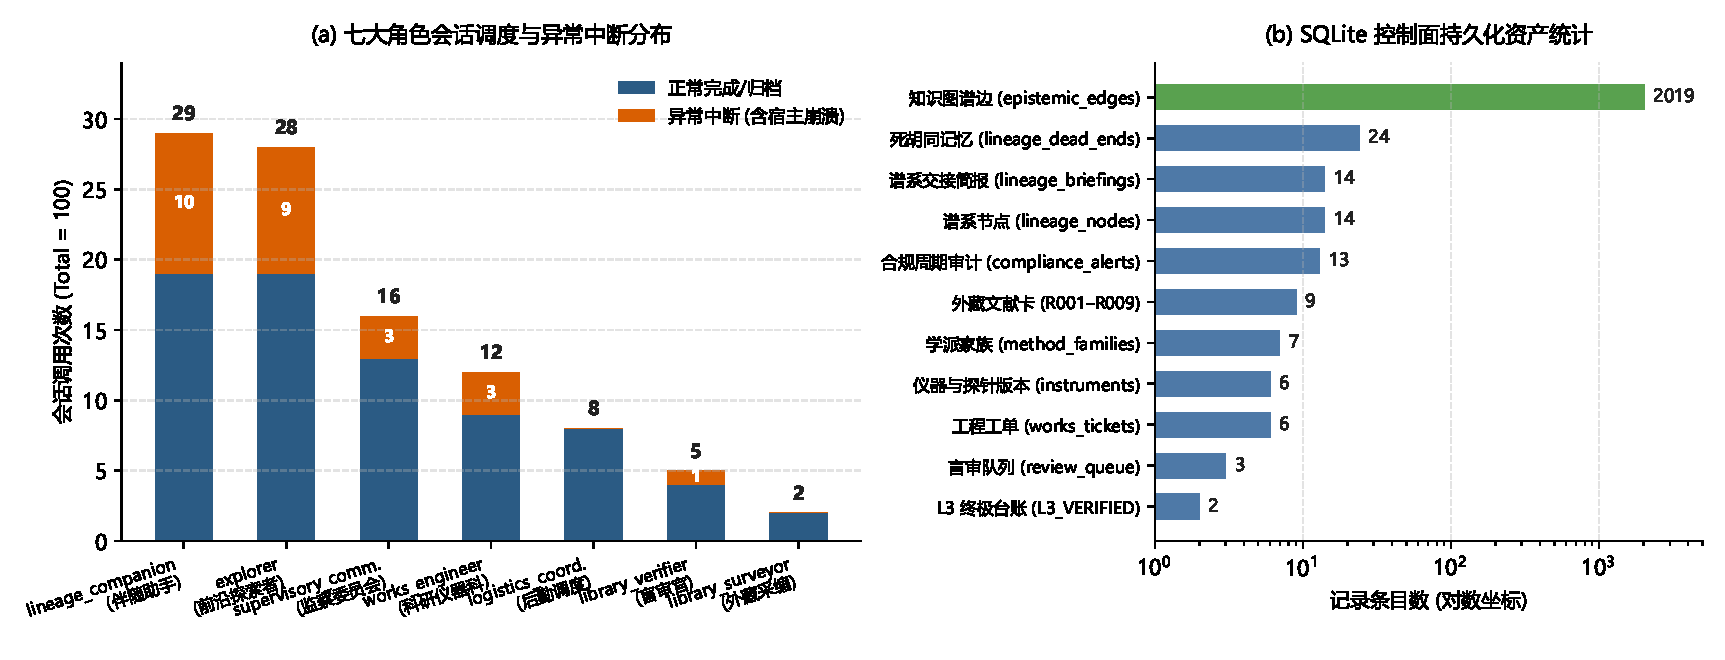
\includegraphics[width=\textwidth]{figures/fig1_telemetry_overview.pdf}
\caption{第 7 轮实机测试系统遥测与控制面资产全景。（a）七大角色 100 次子会话调度与异常中断分布；（b）SQLite 控制面（\texttt{greatwall.db}）各核心表持久化记录规模（对数坐标）。}
\label{fig:telemetry}
\end{figure}

\subsection{元反思效果、工造司贡献与真实交互实录}
\paragraph{1. \texttt{REFLECT\_37} 元反思驱动范式跃迁}
在 \path{b_q1_fam_q1_conve_a9cb7} 分支中，gen1 节点（\path{node_q1_3f3f875f}）早期采用 $3^\circ$ 粗网格生成示向三元组，在 24 条死胡同（\path{de_895b9f39de}）中暴露出“随机组合自洽率仅 0.4\%、失效率严重失真”的陷阱。经 37\% 夜科学元反思与交接后，gen2 节点（\path{node_q1_910faffd}）彻底放弃网格盲扫，转向“以 $(S_1,S_2)$ 基线相似归一化构造 2-环面形状空间 + 物理测度参数化”，最终一举推导出两站精确开带闭式并入账 \path{L3-002}。

\paragraph{2. 科研仪器科（\texttt{works\_engineer}）的四项核心交付}
本轮共调度仪器科 12 次，全面验证了白皮书“以扩张可观测性与防作弊为最高杠杆”的设计思想：
\begin{itemize}
    \item \textbf{自建协议一致模拟器（\path{inst_surrogate_simulator} v1 $\to$ v2）}：18 例校准集 18/18 匹配；额外自设 2 例集外缺陷注入（误差半宽 $1.5^\circ$、测量耗时 $4.0\text{ s}$）均准确捕获 \texttt{OK+FAIL}，证明绝非拟合校准集；1,000 案例 $\times$ 40 动作批量运行仅耗时 $3.29\text{ s}$（303.5 案例/秒）；
    \item \textbf{只读证据摘要探针（\path{probe_worktree_evidence_digest} v1 $\to$ v3）}：针对痛点工单 \path{tkt_9529a8d0e0}，v3 首创剔除约 70 个运行时时钟字段的 \path{canonical_sha256} 规范哈希，彻底消除复跑假阳性；
    \item \textbf{反思字数探针（\path{probe_reflection_budget} v1）}：响应痛点工单 \path{tkt_9d95f3bc19}（反思字数校验不透明），实现 12/12 校准与 22/22 自检，自动分发至 5 个活跃 Worktree；
    \item \textbf{紧急安全护栏组件（\path{evaluators/safety/}）}：受理 P0 工单 \path{WO-B-2026-001} 后连夜编写 \path{safe_sampling.py}、\path{safe_run.py} 与 6 个压力测试夹具。
\end{itemize}

\begin{tcolorbox}[dialoguebox, title={真实交互实录一：隔离盲审沙箱两阶段交锋（\path{review_queue: rev_001}，20:57--20:59）}]
\small
\textbf{[探索者 \path{node_q1_318fa665} A 栏]}：“E1 构造等边三角形反例（$d=58.000\text{ m}, 2r/d=1.1547005384$）；E3 显示 $n=2$ 时 $2r/d\equiv 1$（900 例零反例）；E3b 对抗搜索得 \texttt{max 2r/d=1.00059}，未超过 1；E6 $\Delta=2.001^\circ$ 已塌缩为空。”\\
\textbf{[盲审官 \path{library_verifier} 在空白沙箱 \path{blind_sandbox_rev_001} 独立复算后裁决：REVISE]}：\\
“1. \textbf{【$n=2$ 过泛】}沙箱已构造物理可行反例（$S_1=1200\text{ m}@23.3^\circ, S_2=1100\text{ m}@293.3^\circ$），实测 $2r/d=1.000555895 > 1$，直径圆漏出 $0.9573\text{ m}$；\\
2. \textbf{【算术矛盾】}\texttt{1.00059} 算术上大于 1，不可写『未超过 1』；\\
3. \textbf{【E6 假阴性】}$\Delta=2.001^\circ$ 经 LP 求解存在可行点 $(499.7501, 28630.66)$，区域非空有界（$d=5.727\times 10^7\text{ m}$），并非空集。”
\end{tcolorbox}

\begin{tcolorbox}[dialoguebox, title={真实交互实录二：痛点工单闭环（\path{tkt_9529a8d0e0} $\to$ \path{Obs-001}）与危机裁决（\path{R1}）}]
\small
\textbf{[工单驱动探针演化]}：探索者反馈 JSON 内嵌 \texttt{elapsed\_s} 导致整文件哈希漂移假阳性 $\to$ 仪器科升级 \path{probe_worktree_evidence_digest} v3 引入 \path{canonical_sha256} $\to$ \path{Obs-001} 扫描 30 文件（767 数值字段）实现 \texttt{gaps=0, evidence\_complete=1}。\\
\textbf{[危机处置]}：21:50 Q2 \path{near_edge_out} 触发无界采样致宿主两次崩溃（峰值 20,074\,MB）$\to$ 主控签发 \path{R1} 裁决与 \path{WO-B-2026-001}，撤回曾误杀 ComfyUI（3,106\,MB）的外部看门狗，挂载护栏重启 Q2 双分支继续运行。
\end{tcolorbox}

% =====================================================================
\section{有效科学发现与阶段性产出}
% =====================================================================

\subsection{子题 Q1 的完整科学闭环（L3-001 与 L3-002）}
Q1 通过 \path{rev_002} 与 \path{rev_003} 产出了两项 \path{FULL_GOAL} 级 \path{L3_VERIFIED} 成果：
\begin{itemize}
    \item \textbf{几何载体与旋转卡壳交叉验证}：$\pm 1^\circ$ 示向楔形交会区 $K$ 为至多 $2k$ 条边的闭凸多边形（3,000 例 0 违例），旋转卡壳法~\cite{toussaint1983solving} 与 SciPy 250 例交叉复核直径最大偏差仅 $1.04\times 10^{-9}\text{ m}$，MEC 半径~\cite{welzl1991smallest} 最大偏差 $5.19\times 10^{-10}\text{ m}$；
    \item \textbf{直径圆覆盖性证伪与 Thales 充要判据}：
    \begin{theorem}[Thales 充要判据与 Jung 紧上界]
    设非空有界闭凸多边形 $K$ 直径为 $D$（由对 $(A,B)$ 实现），MEC 半径为 $R_{\min}$~\cite{jung1901ueber}，$\rho = 2R_{\min}/D$。则直径圆覆盖 $K \iff \rho = 1 \iff \forall v \in V(K),\; (v-A)\cdot(v-B)\le 0$。一般情形满足 $1 \le \rho \le 1/\sin\theta_{\max} \le 2/\sqrt{3} \approx 1.1547005384$；若强制同心（圆心固定在直径中点），上界退化为 $\sqrt{3}$，同心代价为 $3/2$。
    \end{theorem}
    物理可达带（1000--1500\,m）内 $L=58\text{ m}$ 等边三角形精确反例测得 $\rho=1.154700538379$（与 $2/\sqrt{3}$ 差 $4.44\times 10^{-16}$），直径圆漏出最远顶点 $21.229\text{ m}$；
    \item \textbf{两站精确开带与物理测度失效率}：如图~\ref{fig:q1_results}(a)，两站失效集精确等于宽 $2\delta$ 的开带 $90^\circ < |\Delta| < 90^\circ + 2\delta$（12,950 例 0 违例），带内闭式 $\rho(\Delta)=1/\sin(\Delta-2\delta)$（$\Delta > \Delta^* \approx 90.04^\circ$）；如图~\ref{fig:q1_results}(b)，物理接收带随机实例中 $k=2..12$ 站失效率由 $0.5\%$--$0.75\%$ 升至 $46.75\%$--$49.25\%$，盲审沙箱复算完全一致。
\end{itemize}

\begin{figure}[htbp]
\centering
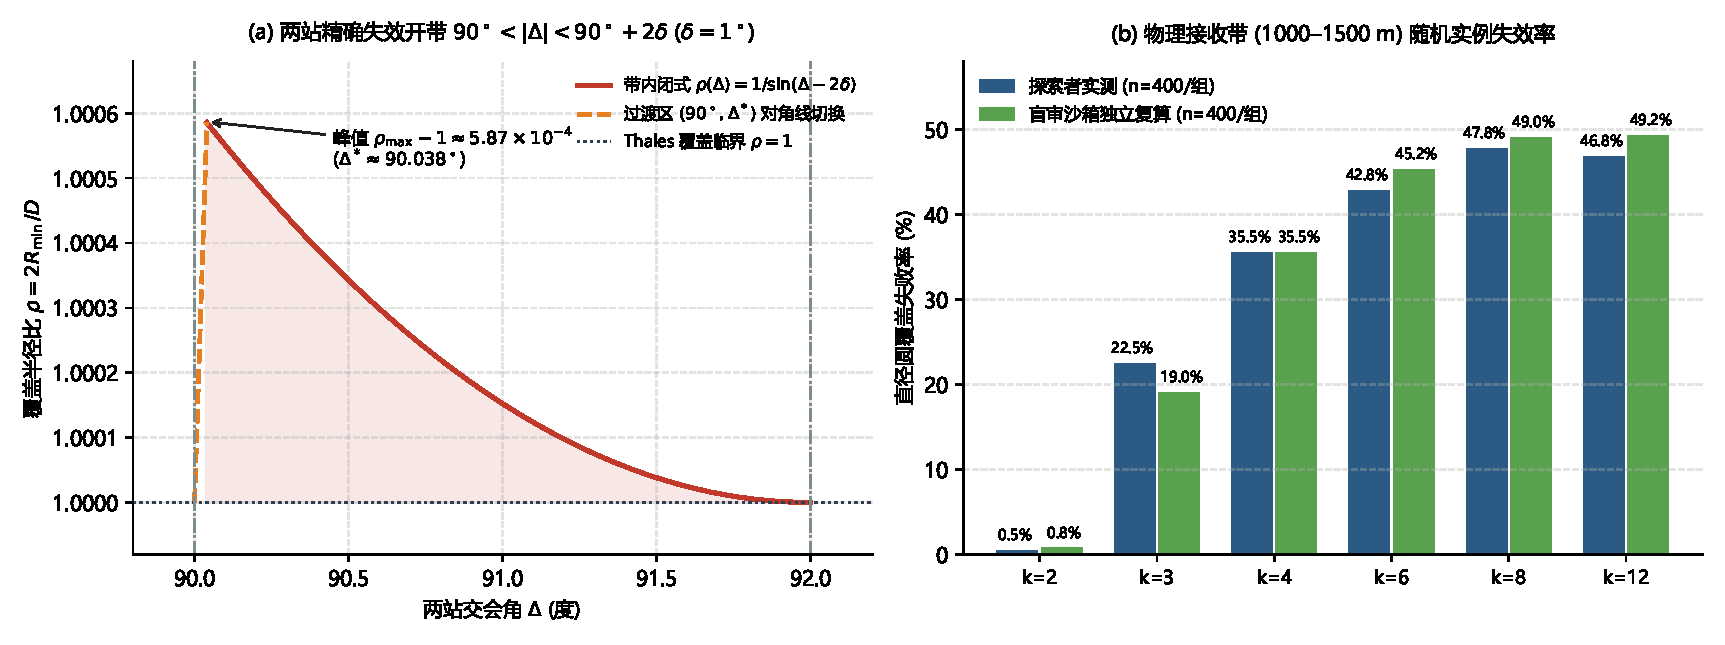
\includegraphics[width=\textwidth]{figures/fig2_q1_empirical_results.pdf}
\caption{Q1 定位区域直径圆覆盖性理论与实测验证。（a）两站精确失效开带理论曲线；（b）物理接收带下 $k=2\text{--}12$ 站随机实例覆盖失败率在探索者与盲审沙箱间的独立复现对比。}
\label{fig:q1_results}
\end{figure}

\subsection{子题 Q2 的阶段性进展}
Q2 两条正交学派在挂载 R1 护栏重启后取得初步定量进展：(1) 贝叶斯期望面积学派~\cite{stansfield1947statistical}（\path{b_q2_fam_q2_bayes_1acfb}）在 \path{exp1_scan_A.json} 中测得单站面积 $A_1=39,269.91\text{ m}^2$ 下最优次站位于 $r=1000\text{ m}, \psi=18^\circ$（$J_{\min}=578.28\text{ m}^2$），\path{exp2_geom_check.json} 交叉验证相对误差 $0.22\%$--$2.41\%$；(2) 极小极大最坏几何学派（\path{b_q2_fam_q2_minim_4872a}）在 \path{exp1_landscape.json} 中测得最优基线 $b^*=1011.43\text{ m}, \psi^*=15.67^\circ$。按 R1.6 口径，上述结果目前仅作阶段性中间资产存档。

% =====================================================================
\section{问题重心剖析与下一步改进方向：聚焦“收敛”与“算力”}
% =====================================================================

本轮测试验证了 V6-Up v3.0 架构的可行性，同时也极其清晰地暴露出当前多智能体长程跑批的\textbf{核心重心问题}——不是系统崩溃，而是\textbf{已达标子题未及时收敛止盈与全局算力额度（Quota/并发）失配}（完整演进链见图~\ref{fig:rca}）。

\begin{figure}[htbp]
\centering
\begin{tikzpicture}[
    node distance=0.5cm and 0.6cm,
    box/.style={rectangle, draw=blue!55!black, fill=blue!4, rounded corners=3pt, text width=3.15cm, align=center, font=\scriptsize, minimum height=1.0cm},
    errbox/.style={rectangle, draw=red!65!black, fill=red!6, rounded corners=3pt, text width=3.2cm, align=center, font=\scriptsize, minimum height=1.0cm},
    govbox/.style={rectangle, draw=teal!60!black, fill=teal!5, rounded corners=3pt, text width=3.2cm, align=center, font=\scriptsize, minimum height=1.0cm},
    arrow/.style={-{Stealth[length=2mm]}, thick, color=gray!60!black}
]
\node[errbox] (n1) {21:50 阶段性事故\\Q2 无界拒绝采样\\峰值 RSS 20,074\,MB 崩溃};
\node[govbox, right=of n1] (n2) {22:13--22:35 修复重启\\R1 护栏 + \texttt{WO-B-2026-001}\\挂载护栏重启恢复并行};
\node[box, right=of n2] (n3) {Q1 与 Q2 并发续跑\\已进入 Q2（2 分支），但 Q1\\仍保留 3 个分支同步空耗};
\node[errbox, below=of n3] (n4) {22:36--22:44 最终停机主因\\触发 5 并发限流与 HTTP 402\\\texttt{Insufficient Balance} 耗尽};
\node[govbox, left=of n4] (n5) {停机影响评估\\若非账户额度耗尽\\修复后的系统本可继续长跑};
\node[govbox, left=of n5] (n6) {第 8 轮核心改进\\Q1 首获 L3 即收敛止盈\\算力集中保障 Q2/Q3/Q4};

\draw[arrow] (n1) -- (n2);
\draw[arrow] (n2) -- (n3);
\draw[arrow] (n3) -- (n4);
\draw[arrow] (n4) -- (n5);
\draw[arrow] (n5) -- (n6);
\end{tikzpicture}
\caption{第 7 轮测试“阶段性资源崩溃 $\to$ 修复重启并发续跑 $\to$ 额度耗尽最终停机”完整演进链。}
\label{fig:rca}
\end{figure}

\subsection{本轮暴露的核心问题重心}
\begin{enumerate}
    \item \textbf{直接终局原因：外部 API 额度耗尽（HTTP 402）与 5 并发限流}：22:13--22:24 修复资源失控并重启 Q2 分支后，系统实际上重新稳定运行并推进了仪器安全层与 Q2 实验。真正截断实验的直接原因是账户余额耗尽：\texttt{22:36:50} 仪器科（\path{gw_works_engineer_2c65036e}）、\texttt{22:38:09} Q2 探索者（\path{gw_exp_node_q2_2d2e06d1_d32a88}，此前已触发 \texttt{concurrency is 5} 限流）与 \texttt{22:44:11} 主控会话（\path{session-435a1e9b}）连续因 \texttt{402 Insufficient Balance} 终止。若非余额耗尽，系统本可继续长跑；
    \item \textbf{根本调度缺陷：已进入 Q2 但 Q1 仍多路并发，未能及时收敛止盈}：Q1 先后入账 \path{L3-001} 与 \path{L3-002} 两项 \path{FULL_GOAL} 级成果后，系统缺乏“子题达标即收敛冻结”机制，仍同时维持 3 个活跃 Q1 分支（\path{suppo_4245e}、\path{certi_c32da}、\path{twost_9c4e1}）与 Q2 双分支并行消耗 Token 与并发槽位（多次 \texttt{free\_slots=0}），导致大量算力额度被已达标的 Q1 冗余分支吞噬，在余额耗尽前未能让 Q2 收敛、亦未能启动 Q3/Q4；
    \item \textbf{遗留工程短板（\path{WO-B-2026-001} 验收待闭环与状态落标延迟）}：\path{evaluators/safety/}（\path{safe_sampling.py}、\path{safe_run.py}）代码已落盘但 8 项验收尚未走完，且 \path{stage1_works_checked=0} 存在状态落标延迟。
\end{enumerate}

\subsection{第 8 轮及长期改进路线：收敛、算力与生态演进}
\begin{enumerate}
    \item \textbf{多题收敛止盈与动态算力配额}：参照station，引入 Supervisor + 周期性元反思：The Station 开放式探索扩展版 专门用 Supervisor 机制 + 周期性 Meta-Reflection 监控各子题的收敛状态，已达标子题自动冻结其 Worktree 并释放算力额度给未达标子题，确保全局算力集中于当前最优攻关方向；
    \item \textbf{算力与资源安全底座闭环}：当前的算力分配存在较大问题，我的api都不够支撑烧测试的；同时安全底座没有设计，提升系统的运行稳定性
    \item \textbf{增强人机协同效能，破解“极简事件簿”权限两难}：当前极简事件簿（控制面与主控）的权限设定陷入两难——权限过高易诱导其越界下场亲自改码干活、破坏隔离制衡；权限过弱则受困于刚性程序状态机，在面对突发异常时难以及时灵活处置。
    \item \textbf{前端 UI 重构与视觉交互体验升级}：目前依托 DSH 原生框架搭建的前端在信息层级、谱系 DAG 动态呈现与美术设计上仍有较大欠缺。后续将重新设计面向科研人员的交互式工作台 UI（涵盖动态谱系演化树、实时算力/Token 燃尽监控、两阶段盲审 Diff 对比及结构化看板可视化），提升长周期实验的可观测性与美观度；
    \item \textbf{科学底座标准化与“标准插座”生态兼容}：进一步打磨通用科学底座，全面基于 \textbf{MCP、Agent Skills 与 Plugin 标准}构建可热插拔的\textbf{“科研标准插座”}。后续将重点借鉴 \textbf{Biomni、Virtual Lab} 等领域专用科研调度框架，深度接入 \textbf{Lean 4} 等形式化数学与定理证明生态，并积极兼容 \textbf{K-Dense-AI、Claude-scientific-skills} 等社区开源科学技能库，实现跨学科工具链的即插即用；但是在开放问题上和真实的科研问题上缺少廉价的Groun-Truth Verifier，导致科研问题的验证成本过高，后续将考虑引入更多的科研验证机制，同时也在考虑面向开放性问题的科研验证机制，提高效果，避免虚假繁荣
    \item \textbf{中央图书馆检索与知识组织持续优化}：进一步打磨图书馆两翼（外藏先验 \texttt{[R\#\#\#]} 与内藏 \texttt{L3/L2}）的 FTS5 语义检索精度、目录卡摘要信息密度及跨代引用剪枝策略，降低探索者在 \texttt{37\%} 解锁后拉取（Pull）文献时的噪声与无效 Token 消耗；
    \item \textbf{拓展科研协作者与前沿文献深度反刍}：积极招募与寻找更多对自主科学发现感兴趣的协作者共同打磨系统；同时持续精读前沿论文、拆解借鉴社区优秀开源项目的工程实践，结合实机测试暴露的短板定期反思并重构本架构的深层局限。
\end{enumerate}

% =====================================================================
% 参考文献
% =====================================================================
\bibliographystyle{plain}
\bibliography{references}

\end{document}
